% ju 14-5-22
\section*{Einleitung}

\emph{Sonderzeichen}  wie >>\& oder \%<< müssen mit einem Backslash \verb|\& oder \%| maskiert werden, 
damit sie von LaTeX nicht als Befehle missverstanden werden.

Tabellenbuch (\textcite{bell:2021:tabellenbuchKfz} S. 281)

\emph{Website} \footnote{\url{https://golatex.de/wiki/Hauptseite}} \verb|\footnote{\url{https://golatex.de/wiki/Hauptseite}}| 


\clearpage
\subsection*{Stand der Forschung}

Während die traditionelle Latexproduktion bereits hinreichend erforscht ist (\autoref{fig:latex}) \\
\verb|(\autoref{fig:latex})|, bleibt das wissenschaftliche Verständnis elektronischer Verarbeitungsprozesse dieses 
vielseitigen Materials weiterhin lückenhaft. 


\begin{figure}[!h]% hier: !ht
	\centering
	
\includegraphics[width=0.25\textwidth]{images/Logo/logo.eps}
	\caption{Traditionelle Latexproduktion}\label{fig:latex}%
\end{figure}

\clearpage
\section*{Ausblick}

Daraus ergeben sich gemäß (\autoref{tab:schritte}) \verb|(\autoref{tab:schritte})| folgende nächste Schritte, 
deren sequenzielle Ausführung von essenzieller Bedeutung ist.

\begin{table}[!h]% hier: !ht
	\centering
	\begin{tabular}{@{}cl@{}}% lcr
		\toprule
		\textbf{Nr.} & \textbf{Vorgehen} \\
		\midrule
		1 & Aktuellen Forschungsstand recherchieren \\
		2 & Methoden entwickeln \\
		3 & Schlussfolgerung aufstellen \\
		\bottomrule
	\end{tabular}
	\caption{Nächste Schritte}\label{tab:schritte}
\end{table}

\clearpage
\section*{Listen}%\label{sec:listen}\index{Listen}
	% Checkliste
	\begin{itemize}[label=\checkmark] %\itemsep -2pt
		\item Check
	\end{itemize}

	% Checkliste
	\begin{itemize} 
		\item [$\square$] Check
	\end{itemize}

	% Liste
	\begin{itemize} 
		\item Punkt
	\end{itemize}
	% Liste numeriert
	\begin{enumerate} 
		\item Liste numeriert
		\item Punkt
	\end{enumerate}

\clearpage
\section*{Abbildungen}%\label{sec:Abbildungen}\index{Abbildungen}

	Liste

	\begin{itemize} 
		\item Punkt
		\item Punkt
		\item Punkt
		\item Punkt
	\end{itemize}
			
	\begin{figure}[!h]
	\centering
	\subcaptionbox{Logo 1 \label{logo1}}
	{
\includegraphics[width=0.25\textwidth]{images/Logo/Logo1}}
	\subcaptionbox{Logo 2 \label{logo2}}
	{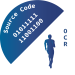
\includegraphics[width=0.25\textwidth]{images/Logo/Logo2}}
	\caption{Zwei Logos}\label{Logos}
	\end{figure}

\clearpage
\section*{Abbildungen 2}%\label{sec:Abbildungen2}\index{Abbildungen2}
	%Logo in Neg, Grau, Schwarz (\autoref{fig:logoneggrauschwarz}).
	%
	\begin{figure}[!h]% hier: !hb
		\centering
		\begin{minipage}[b]{0.40\textwidth}
			
\includegraphics[width=\textwidth]{images/Logo/Logo-negativ}%
		\end{minipage}
		\hfill
		\begin{minipage}[b]{0.30\textwidth}
			
\includegraphics[width=\textwidth]{images/Logo/Logo-Grau}%
		\end{minipage}
		\hfill
		\begin{minipage}[b]{0.20\textwidth}
			
\includegraphics[width=\textwidth]{images/Logo/Logo-SW}%
		\end{minipage}
		\caption{Logo in Neg, Grau, Schwarz}\label{fig:logoneggrauschwarz}%% anpassen
	\end{figure}

\clearpage
\section*{Text und Abbildungen}%\label{sec:TAbbildungen}\index{Text, Abbildungen}
	%Logo in Neg, Grau, Schwarz (\autoref{fig:logoneggrauschwarz}).
	%
	\begin{figure}[!h]% hier: !hb
		\centering
		\begin{minipage}[c]{0.55\textwidth}
			Liste
			\begin{itemize} 
				\item Punkt
				\item Punkt
				\item Punkt
				\item Punkt
			\end{itemize}
		\end{minipage}
		\hfill
		\begin{minipage}[c]{0.35\textwidth}
			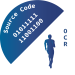
\includegraphics[width=\textwidth]{images/Logo/Logo2}%
		\end{minipage}
		%\caption{Logo in Neg, Grau, Schwarz}\label{fig:logoneggrauschwarz}%% anpassen
	\end{figure}

\clearpage
\section*{Tabelle}%\label{sec:Tabelle}\index{Tabelle}

	\begin{table}[!h]% hier: !ht 
		\centering
		\caption{\textbf{Integer-Datentypen}}
		\label{tab:Integer-Datentypen}
		\begin{tabular}{@{}lll@{}}
		\toprule
		\textbf{Typ}       & \textbf{Wertebereich}    & \textbf{Speicherbedarf} \\ \midrule
		int                & –32768...32767           & 2 Bytes                 \\
		int                & –2147483648...2147483647 & 4 Bytes                 \\
		short int          & –32768...32767           & 2 Bytes                 \\
		unsigned short int & 0...65535                & 2 Bytes                 \\
		long int           & -2147483648...2147483647 & 4 Bytes                 \\
		unsigned long int  & 0...4294967295           & 4 Bytes                 \\ \bottomrule
		\end{tabular}%
	\end{table}


